\documentclass{article}

\PassOptionsToPackage{numbers, sort, compress}{natbib}
\usepackage[main,final]{neurips_2025}

\usepackage[T1]{fontenc}
\usepackage[utf8]{inputenc}
\usepackage{hyperref}
\usepackage{url}
\usepackage{booktabs}
\usepackage{nicefrac}
\usepackage{microtype}
\usepackage{xcolor}

%%%

\usepackage{subcaption}
\usepackage{graphicx}
\usepackage{multirow}
\usepackage{amsmath,amssymb,amsfonts}
\usepackage{amsthm}
\usepackage{mathrsfs}
\usepackage{xcolor}
\usepackage{textcomp}
\usepackage{manyfoot}
\usepackage{algorithm}
\usepackage{algorithmicx}
\usepackage{algpseudocode}
\usepackage{listings}

\graphicspath{{../slides/figs/}}

\newtheorem{theorem}{Theorem} % continuous numbers
%%\newtheorem{theorem}{Theorem}[section] % sectionwise numbers
%% optional argument [theorem] produces theorem numbering sequence instead of independent numbers for Proposition
\newtheorem{proposition}[theorem]{Proposition}%
\newtheorem{lemma}{Lemma}%
%%\newtheorem{proposition}{Proposition} % to get separate numbers for theorem and proposition etc.

\newtheorem{example}{Example}
\newtheorem{remark}{Remark}

\newtheorem{definition}{Definition}
\newtheorem{assumption}{Assumption}

%%%


\title{Estimating the Direction of Motion of a Moving Object from Monocular Video Using Inertial Sensor Data}


% The \author macro works with any number of authors. There are two commands
% used to separate the names and addresses of multiple authors: \And and \AND.
%
% Using \And between authors leaves it to LaTeX to determine where to break the
% lines. Using \AND forces a line break at that point. So, if LaTeX puts 3 of 4
% authors names on the first line, and the last on the second line, try using
% \AND instead of \And before the third author name.


\author{
  Matvey Glazunov\\
  Lomonosov Moscow State University\\
  Moscow, Russia\\
  \texttt{email@example.com}\\
  \And
  Maxim Kryzhanovsky (consultant)\\
  Moscow, Russia\\
  \texttt{email@example.com}\\
  \And
  Konstantin Vorontsov (advisor)\\
  Lomonosov Moscow State University\\
  Moscow, Russia\\
  \texttt{email@example.com}\\
}


\begin{document}


\maketitle

\begin{abstract}
    We consider the problem of estimating the direction of motion of a moving object from a monocular onboard camera and inertial sensors. The translation direction is visible in the image as the focus of expansion and is usually recovered from the essential matrix of two frames. Such an estimate is noisy, lags behind after smoothing, and breaks down on degenerate frames: low parallax, a dominant plane, fast rotation. We combine the visual measurement with gyroscope and accelerometer data in a complementary filter on the unit sphere. The filter works in the body frame and does not use heading, which is unreliable in our recordings. In experiments on one recorded sequence, split into a tuning window and a separate validation window, the filter reduces the delay of the vision-only channel from 333--367\,ms and 567--633\,ms to 67--200\,ms and 0--133\,ms respectively. Jitter is lower on the horizontal angle in both windows; on the vertical angle it is 12\% higher on the tuning window and 26\% lower on the validation window. We plan to add a learned estimate of the reliability of the visual measurement and to compare the method with three baselines: a vision-only essential-matrix pipeline, vision with rotation taken from the gyroscope, and the visual-inertial odometry system OpenVINS.
\end{abstract}

\textbf{Keywords:} direction of motion, focus of expansion, essential matrix, visual-inertial fusion, complementary filter, gyroscope.

\section{Introduction}\label{sec:intro}

The direction of motion of a moving object is needed by control and navigation systems: it allows holding a course, estimating drift and stabilizing the object. When a camera moves, image points diverge from a single point, the focus of expansion (FOE), which defines the direction of translation in the camera frame~\citep{longuet1980interpretation}. We estimate this direction from monocular video and inertial sensors in real time.

The classical approach recovers motion from the essential matrix of two frames, using five points~\citep{nister2004five} and rejecting outliers with RANSAC~\citep{fischler1981ransac}. For noisy optical flow, confidence weights have been proposed~\citep{jaegle2016egomotion}. Velocity and angular velocity are estimated from the flow and the inertial sensors by filters and observers~\citep{grabe2015nonlinear, zhong2020direct}, and velocity can be estimated without recovering the pose~\citep{xu2024tight}. Rotation known from a gyroscope simplifies the geometry and helps to reject outliers~\citep{kneip2011robust, troiani2014twopoint}. Full visual-inertial systems give reference accuracy~\citep{geneva2020openvins}.

A vision-only estimate is noisy, contains rare outliers and lags behind after smoothing. It degenerates in the presence of a dominant plane~\citep{chum2005dominant}, and the FOE is poorly observable where the flow near the point of expansion is weak~\citep{dinaux2021faith}. In methods with known rotation, the gyroscope works inside the geometric step, so the resulting channel remains a visual one with all its delay. A full visual-inertial system requires raw inertial data and a camera--IMU calibration and estimates the whole state, while only the direction is needed.

We lead the direction by a complementary filter on the unit sphere in the body frame. The gyroscope and the accelerometer describe the dynamics between frames, and the visual measurement slowly pulls the estimate. Heading is not used, because it is unreliable in our recordings. The weight of the visual measurement is planned to be obtained from a learned estimate of its reliability~\citep{yi2018learning, qiu2023airimu}.

\textbf{Contributions.} Our contributions can be summarized as follows:
\begin{itemize}
    \item We state the problem of estimating the direction of motion without heading (Section~\ref{sec:prelim}).
    \item We use a complementary filter on the sphere~\citep{mahony2008nonlinear, kurz2017libdirectional} and measure its delay and jitter against a zero-phase reference (Section~\ref{sec:exp}).
    \item We report experiments on recordings of a moving object, with a separate validation window. To the best of our knowledge, a close problem statement without heading and with a separate measurement of the channel delay is not covered in the literature we reviewed.
\end{itemize}

\textbf{Outline.} Section~\ref{sec:rw} reviews related work, Section~\ref{sec:prelim} gives the notation and the problem statement, Section~\ref{sec:method} describes the method, Section~\ref{sec:exp} reports the experiment.

\section{Related Work}\label{sec:rw}

\textbf{Ego-motion and the focus of expansion.} The decomposition of the optical flow into translational and rotational parts goes back to~\citet{longuet1980interpretation}. \citet{jaegle2016egomotion} weight noisy flow measurements by confidence; \citet{dinaux2021faith} estimate the FOE with RANSAC from event-based flow and show that it is poorly observable near the point of expansion. Velocity and angular velocity are estimated from optical flow with an inertial sensor in~\citep{grabe2015nonlinear}, and directly by an iterated Kalman filter in~\citep{zhong2020direct}. \citet{xu2024tight} estimate velocity directly without recovering the pose, and \citet{lee2017forward} use the IMU to derive feature confidence for forward motion.

\textbf{Two-view geometry and degeneracy.} The five-point solver~\citep{nister2004five} with RANSAC~\citep{fischler1981ransac} is the standard way to obtain the essential matrix. RANSAC fails when a dominant plane is present~\citep{chum2005dominant}. A rotation known from a gyroscope reduces the problem to estimating the translation direction~\citep{kneip2011robust}, and two correspondences and the gyroscope are enough to reject outliers~\citep{troiani2014twopoint}.

\textbf{Visual-inertial fusion.} OpenVINS~\citep{geneva2020openvins} is a filter-based open platform that also calibrates the camera--IMU time offset; it serves as a full-system reference.

\textbf{Filtering on manifolds.} Complementary filters on the rotation group~\citep{mahony2008nonlinear} and recursive filters on the unit sphere with von~Mises--Fisher and Bingham distributions~\citep{kurz2017libdirectional} give the theoretical basis for filtering a unit vector.

\textbf{Learned measurement confidence.} A network can label correspondences as inliers or outliers~\citep{yi2018learning}, predict the uncertainty of an inertial sensor~\citep{qiu2023airimu}, or learn the reliability of visual measurements without ground truth, using multi-view consistency as self-supervision~\citep{choi2025statistical}; neural measurement covariances have been proposed for visual-inertial odometry with unreliable vision~\citep{guo2026lbdu}.

\textbf{Evaluation.} Alignment and error metrics for visual-inertial odometry are given in~\citep{zhang2018tutorial}; we need an analogous metric for the direction of motion.

\section{Preliminaries}\label{sec:prelim}

\subsection{General notation}

For each frame $k=1,\dots,N$ we use: $z_k$ is the visual direction of motion, a unit vector obtained from a pair of frames; $\hat d_k(\theta)$ is the estimate of the direction produced by a filter with parameters $\theta$; $\bar z_k$ is the reference, the raw visual measurement smoothed by a symmetric window; $\tau(\theta)$ is the delay of the estimate; $J(\theta)$ is its jitter; $J_{\mathrm{vis}}$ is the jitter of the vision-only estimate. The direction is expressed by two angles relative to the optical axis, horizontal and vertical; the delay and the jitter are computed for each angle separately.

\subsection{Assumptions}

The scene is rigid; the visual measurement equals the true direction plus noise with rare outliers; the gyroscope bias is small over a fraction of a second; heading is not used. The speed of the object is taken from an external source.

\subsection{Problem statement}\label{sec:problem}

\textbf{Given.} For each frame: a video frame, gyroscope and accelerometer readings, roll and pitch.

\textbf{Find.} The direction of motion $\hat d_k$ of the object in its body frame, for each frame.

\textbf{Model.} A filter $F_\theta$ that outputs $\hat d_k(\theta)$. The parameters $\theta$ are the strength of the correction by vision, the length of the median window and the threshold for rejecting outliers.

\textbf{Criterion.} The delay is the time shift at which the estimate is closest to the reference:
\begin{equation}\label{eq:delay}
    \tau(\theta) = \arg\min_{s \ge 0} \Bigl( \tfrac{1}{N} \sum_{k} \bigl(\hat d_k(\theta) - \bar z_{k-s}\bigr)^2 \Bigr)^{1/2},
\end{equation}
and the jitter is the root mean square of the time derivative of the estimate,
\begin{equation}\label{eq:jitter}
    J(\theta) = \Bigl( \tfrac{1}{N} \sum_{k} \bigl( (\hat d_k(\theta) - \hat d_{k-1}(\theta)) / \Delta t \bigr)^2 \Bigr)^{1/2}.
\end{equation}
The task is
\begin{equation}\label{eq:argmin}
    \theta^* = \arg\min_{\theta:\, J(\theta) \le J_{\mathrm{vis}}} \tau(\theta).
\end{equation}
In words: remove the delay without adding jitter.

\section{Method}\label{sec:method}

TODO (to be written after the problem statement is agreed): hypotheses, model, criterion and algorithm of the filter on the unit sphere.

\section{Experiments}\label{sec:exp}

\textbf{Goal.} To check that a complementary filter with a gyroscope reduces the delay of the visual channel of the direction of motion compared with the vision-only pipeline without increasing jitter, and to find out under which parameters this holds.

\textbf{Data.} One recorded sequence of a moving object: video $1200\times900$ at 30 frames per second, telemetry at about 192\,Hz (roll, pitch, angular rates, speed from an onboard estimator), synchronized with the video by cross-correlation of the direction of motion. The sequence is split into a tuning window (60--160\,s, 3002 frames) and a validation window (160--260\,s, 3002 frames), on which the parameters were not tuned. The recording is not publicly available; an open dataset with ground truth is planned (Section~\ref{sec:plan}).

\textbf{Baseline.} The vision-only pipeline \texttt{foe\_pose}: Shi--Tomasi corners, pyramidal Lucas--Kanade with a forward-backward check, the essential matrix with RANSAC and \texttt{recoverPose}, smoothing with a weight by the number of inliers, and a limit on the angular rate. The image is resized to 640 pixels in width, the frame gap is 15 frames. Configuration: \texttt{code/configs/foe\_pose.json}.

\textbf{Filter parameters.} Correction rate $8\,\mathrm{s}^{-1}$, median over the last 5 measurements, gate $45^\circ$, accelerometer on, speed magnitude from the onboard estimator. Configuration: \texttt{code/configs/experiment.json}.

\textbf{Reproduction.} \texttt{python code/run\_experiment.py} runs both windows and writes the numbers and the figure; the video and the telemetry paths are set in the configuration.

\subsection{Preliminary results}

\begin{figure}[t]
    \centering
    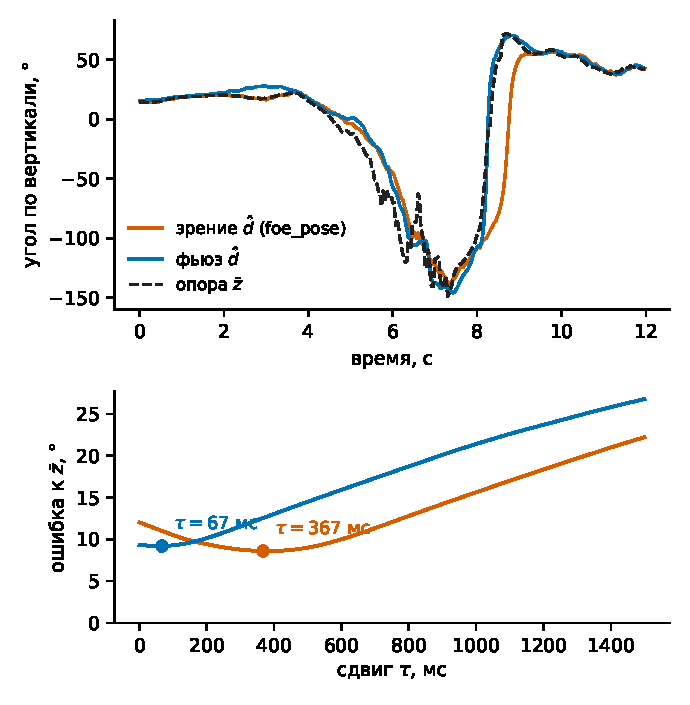
\includegraphics[width=0.55\textwidth]{main_figure.pdf}
    \caption{Tuning window, vertical angle. Top: the reference $\bar z$ (dashed), the vision-only estimate (orange) and the filter output (blue) over 12 seconds; the vision-only estimate lags behind at the fast turn. Bottom: RMS difference to the reference as a function of the time shift $\tau$; the minimum of each curve is the delay of the channel: 367\,ms for vision, 67\,ms for the filter.}
    \label{fig:main}
\end{figure}

\begin{table}[t]
    \centering
    \caption{Delay, jitter and RMS difference to the reference, horizontal ($x$) / vertical ($y$) angle. Raw measurement jitter: 471/727 (tuning), 385/559 (validation) deg/s.}
    \label{tab:results}
    \begin{tabular}{llccc}
        \toprule
        Window & Channel & Delay, ms & Jitter, deg/s & RMS to reference, deg \\
        \midrule
        \multirow{2}{*}{tuning}     & vision only & 333 / 367 & 25.0 / 35.7 & 6.0 / 8.6 \\
                                    & with filter & 200 / 67  & 20.2 / 40.0 & 6.0 / 9.2 \\
        \midrule
        \multirow{2}{*}{validation} & vision only & 633 / 567 & 24.6 / 29.5 & 8.2 / 8.9 \\
                                    & with filter & 0 / 133   & 19.7 / 21.9 & 15.3 / 18.0 \\
        \bottomrule
    \end{tabular}
\end{table}

Figure~\ref{fig:main} and Table~\ref{tab:results} show that the filter reduces the delay on both windows and on both angles. On the tuning window the RMS difference to the reference is the same as for vision; on the validation window it grows from about 9 to 15--18 degrees, so the gain in time is paid for by a larger deviation from the reference. The reason has not been established yet: it can be the drift of the inertial integral or the noise of the reference itself, which is the raw measurement smoothed over nine frames and still contains outliers.

\subsection{Plan of the experiments}\label{sec:plan}

\begin{enumerate}
    \item Base experiment: the vision-only pipeline on the recording, delay and jitter (done, Table~\ref{tab:results}).
    \item Comparison with the baselines: the raw channel (B1), vision with rotation from the gyroscope (B2), OpenVINS (B3, if raw inertial data are available), the filter.
    \item Analysis: dependence on the correction rate, the median window and the gate; the role of the accelerometer; frames with a body rotation larger than $6^\circ$; sensitivity to calibration errors and to degraded sensors; computational cost.
\end{enumerate}

\section{Discussion}\label{sec:disc}

TODO.

\section{Conclusion}\label{sec:concl}

TODO.


%%%%%%%%%%%%%%%%%%%%%%%%%%%%%%%%%%%%%%%%%%%%%%%%%%%%%%%%%%%%

\bibliographystyle{unsrtnat}
\bibliography{references}

%%%%%%%%%%%%%%%%%%%%%%%%%%%%%%%%%%%%%%%%%%%%%%%%%%%%%%%%%%%%

\newpage
\appendix
\section{Appendix / supplemental material}\label{app}

\subsection{Additional experiments / Proofs of Theorems}\label{app:exp}

TODO

\end{document}
